\section{Plan}
In this section, I will outline a brief outline of my intended plan of action, which will likely be reformed later on as other issues
become more present during the development process.

\subsection{Time Management:}
\begin{figure}[h]
    \centering
    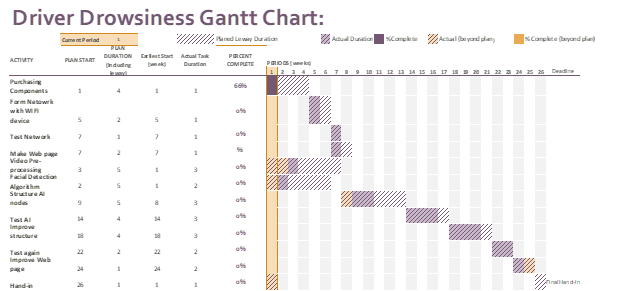
\includegraphics[width=0.9\textwidth]{Images/Gantt_chart.png}
\end{figure}

Here week one refers to the starting week (w/c 20.10.2025) and week 26 being the week of the deadline (w/c 20.04.2025).
The initial delay in this project is due to shipping of components. Since I do not have any of the components that I need to do this
project, I will have to order them, and this takes time. However, in the meantime, I can request permission for datasets as well as
gather a better understanding of what attributes can affect a driver’s concentration and different potential models that I could use for
my lightweight AI component.

\subsection{Connections:}
Since raspberry pie 4 is WIFI compatible, I plan to connect the user’s own device by this. Therefore, using the pi as a host device for
a website that can display data and other information to the user. This is the ideal option as wired displays either require the pi to be:
\begin{itemize}
    \item Dashboard mounted due to a small wire. This has the potential to fall or move, causing further irritation or distraction for
    the driver. This is against the aim of the project of keeping the driver focused on the road.
    \item More wires and additional screens for setting up. Once again, this takes up space in their field of vision and will create
    added hassle if setting up for different drivers. Most people will likely opt to not use this device, making it a futile construction.
\end{itemize}
By using the users’ own wireless device, you not only remove the added expense of the screen (if released to the commercial market) but
also remove clutter. Users are likely to already have phone mounts in their desired location, so why not give the idle device some added
functionality. This will also be optional, if they are already using the device for maps, it will not prevent the system from relaying
information or alerting the user.

\begin{figure}[H]
    \centering
    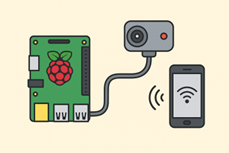
\includegraphics[width=0.7\textwidth]{Images/pie_idea.png}
    \captionsetup{labelformat=empty}
    \caption{\tiny (ChatGPT generated –> prompt=”please make this look nice + drawing of this”)}
\end{figure}
